\documentclass{article}
\usepackage{mystyle}

\title{Notes on x-ray wave-field forward model}
\author{Scott Trinkle}
\date{Last edited: \today}

\begin{document}
\maketitle

\section*{Introduction}
In these notes, I follow the various derivations in Paganin\cite{paganin}
chapters 1 and 2, tracing the propagation of a coherent x-ray wavefield through
a scattering object and to a detector. The goal is to write down a physical
imaging forward model that is as rigorous as possible, in order to simulate
and/or predict the phase effects we have observed in our high-absorbing samples.

This problem will be addressed in two stages:
\begin{enumerate}
\item Propagation of an incoming synchrotron x-ray wave-field $\Psi(x,y,z,t)$
  through a scattering object with frequency-dependent, complex index of
  refraction $n_{\omega}(x,y,z)$ that exists between planes $z=0$ and
  $z=z_0$ along the optical axis, $z$.
\item Propagation of the scattered wave-field from the exit-plane $z=z_0$ to the
  detector plane $z=z_0 + \Delta$, and calculation of the detected intensity:
  $I(x,y,z_0+\Delta) = |\Psi(x,y,z=z_0+\Delta)|^2$
\end{enumerate}

In these notes, I am restricting myself to modeling a single 2D projection of
the object, which I leave in terms of the complex, 3D index of refraction:
$n_{\omega}(x,y,z)$ for now.\footnote{See Appendix~\ref{refractindex} for a
  discussion of the relationship between $n_{\omega}(x,y,z)$ and additional
  physical parameters} The extension to 3D tomographic imaging will be explored
later (I expect that existing tomographic techniques will generally be
appropriate once we understand the 2D phase effect). Note that these notes will
also neglect the effects of incoherent scattering.

I will document all simplifying approximations and assumptions made in the
various derivations presented in these notes. The results will be used to
construct a computational framework that can simulate imaging of realistic
digital phantoms in various imaging geometries. These studies can be used to
understand the validity of different assumptions for our imaging task, which
will be useful as we go on to look at appropriate ways of linearizing and
inverting our model.



\section{Propagation through matter}\label{matter}
In this section, we consider the propagation of an incoming, complex
monochromatic wave-field $\psiom(x,y,z)$ from left to right through an object
parameterized by the frequency-dependent complex index of refraction
$n_{\omega}(x,y,z)$ (the extension to polychromatic wave-fields is discussed in
section~\ref{helmholtz} below). Figure~\ref{fig:proj} illustrates the scattering
geometry to be used throughout these notes.

\begin{figure}[h]
  \centering
  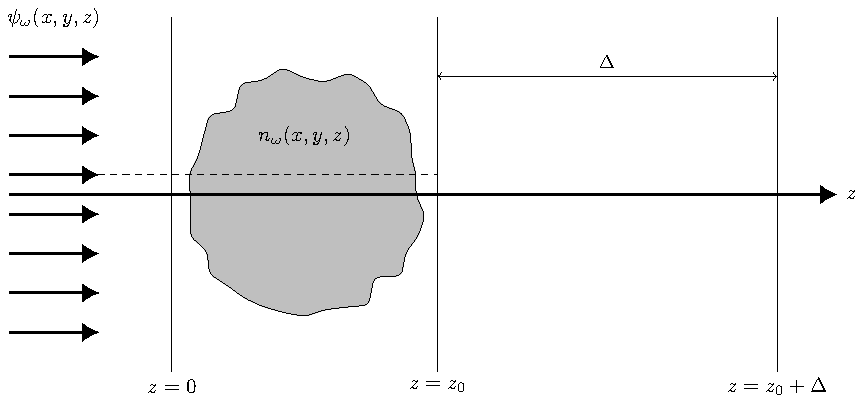
\includegraphics{figs/projfig}
  \captionsetup{width=0.6\linewidth}
  \caption{A $z$-directed monochromatic plane wave $\psiom$ is indicated
    by the arrows at the left of the diagram. All scatterers lie between $z=0$
    and $z=z_0$.}
  \label{fig:proj}
\end{figure}

\subsection{Inhomogeneous Helmholtz equation}\label{helmholtz}
In section 2.1, Paganin starts with Maxwell's equations and develops the
relevant scalar wave equation in the presence of scatterers. A number of typical
assumptions are made; I am listing them here, indexed by the relevant equation
number:

\begin{itemize}
\item (2.5--2.8) The scattering material is linear and isotropic. That is:
  $\bm{D} = \epsilon\bm{E}$ and $\bm{B} = \mu\bm{H}$ where $\bm{D}$ is the
  electric displacement, $\bm{B}$ is the magnetic induction, $\bm{E}$ is the
  electric field, $\bm{H}$ is the magnetic field, $\epsilon$~is the electric
  permittivity and $\mu$ is the magnetic permeability. This assumptions thus
  excludes ferroelectric and ferromagnetic materials, for example.

\item (2.13) The material is static, so both $\mu$ and $\epsilon$ are both
  independent of time.

\item (2.18--2.19) The material is non-magnetic, that is: $\mu(x,y,z) = \mu_0$,
  where $\mu_0$ is the permeability of free space. In other words, we assume our
  metal stains have very low magnetic susceptibility. I am assuming this is a
  fair, typical assumption for most x-ray imaging tasks --- a cursory Wikipedia
  search puts the susceptibility of osmium at $11 \times 10^{-6}$~cm$^{-3}$/mol,
  which seems relatively low compared to other listed metals (aluminum is at
  1.7$\times 10^{-5}$~cm$^{-3}$/mol, for instance).

\item (2.18--2.19) There are no charge or current densities: $\rho(x,y,z,t) = 0$
  and $\bm{J}(x,y,z,t) = \bm{0}$.

\item (2.20--2.21) Scatterers are ``sufficiently slowly varying'' over length
  scales comparable to the wavelength of the x-ray radiation. At 20 keV, our
  wavelength is around $6\times 10^{-11}$ m --- it is fair to assume our samples
  are slowly varying over this length scale.
\end{itemize}

Under these assumptions, a complex scalar, electromagnetic wave $\Psi(x,y,z,t)$ can
be represented as a Fourier integral over non-negative angular frequencies $\omega$:
\begin{align}
  \Psi(x,y,z,t) = \frac{1}{\sqrt{2\pi}}\int_0^{\infty} \psiom(x,y,z)\text{ exp}\left(-i\omega t\right)\mathrm{d}\omega,
  \label{eq:polychromatic}
\end{align}
whose spatial monochromatic components $\psiom(x,y,z)$ obey the
``inhomogeneous'' Helmholtz equation:
\begin{align}
  \label{eq:helm}
  \left[\nabla^2 + k^2 n_{\omega}^2(x,y,z)\right]\psiom(x,y,z) = 0,
\end{align}
where $k$ is the wavenumber ($2\pi/\lambda$) and $n_{\omega}(x,y,z)$ is the
complex, frequency-dependent refractive index of the scatterer, given by:
\begin{align}
  n_{\omega}(x,y,z) = c\sqrt{\epsilon_{\omega}(x,y,z)\mu_0} = \sqrt{\frac{\epsilon_{\omega}(x,y,z)}{\epsilon_0}}.
\end{align}

It is appropriate, then, to develop solutions to equation~\ref{eq:helm} for each
monochromatic component $\psiom$, then use equation~\ref{eq:polychromatic} to
construct the full wave-field. This will be the strategy throughout these
notes. The remainder of this section will detail a number of methods for solving
this equation under different approximations.

\subsection{Projection approximation}

In section 2.2, Paganin reviews the projection approximation. With reference to
Figure~\ref{fig:proj}, we use a cartesian coordinate frame and consider a
monochromatic plane wave $\psiom(x,y,z)$ propagating from left to right along
the optical axis $z$. The object exists within the space $0 < z < z_0$, with all
other space being vacuum. In a ray optics framework, the projection
approximation assumes that ``the scatterers are sufficiently weak so as to
negligibly perturb the ray paths which would have existed in the volume occupied
by the scatterer had the scatterer been absent.'' Effectively, the phase and
amplitude of the disturbance at the surface $z=z_0$ can be expressed in terms of
the phase and amplitude shifts accumulated along a given ray path connecting the
entrance and exit surfaces, with the ray paths being the same as if the
scattering object was absent (one such path is illustrated by the dotted line
through the object in Figure~\ref{fig:proj}).

We begin by modeling the wave as the product of an unscattered plane wave
$\exp(ikz)$ with an envelope $\tilde{\psi}_{\omega}(x,y,z)$:
\begin{align}
  \psiom(x,y,z) = \tilde{\psi}_{\omega}(x,y,z)\exp(ikz),
  \label{eq:envelope}
\end{align}
noting that $|\tilde{\psi}_{\omega}(x,y,z)|^2 =
|\psiom(x,y,z)|^2$. Equation~\ref{eq:helm} can then be expanded in terms of the
envelope $\tilde{\psi}_{\omega}$:
\begin{align}
  \left\{2ik\frac{\partial}{\partial z} + \nabla_{\perp}^2 + \frac{\partial^2}{\partial z^2} + k^2\left[n_{\omega}^2(x,y,z) - 1\right]\right\}\tilde{\psi}_{\omega}(x,y,z) = 0,
  \label{eq:helm2}
\end{align}
where
\begin{align}
  \nabla^2_{\perp} \equiv \frac{\partial^2}{\partial x^2} + \frac{\partial^2}{\partial y^2}
\end{align}

The development of the projection approximation then rests on the following
assumptions:
\begin{itemize}
\item We can neglect the $\partial^2/\partial z^2$ term in equation \ref{eq:helm2}.
  This amounts to the paraxial approximation, which I believe is fair for our
  synchrotron beam.

\item We can also neglect the $\nabla^2_{\perp}$ term, as this is the only
  term that couples neighboring ray trajectories. Paganin does not go into
  any more detail on the conditions under which this is valid, besides
  that we are assuming ``the scattering is sufficiently weak.''
\end{itemize}

From here, we can solve equation~\ref{eq:helm2} and write the wave-field at the
exit surface $z=z_0$ in terms of that at the entrance surface $z=0$:
\begin{align}
  \tilde{\psi}_{\omega}(x,y,z_0) \approx \exp\left\{\frac{k}{2i}\int_0^{z_0} \left[1 - n_{\omega}^2(x,y,z)\right] \mathrm{d}z\right\}\tilde{\psi}_{\omega}(x,y,z=0).
  \label{eq:236}
\end{align}

Define the complex, 2D projection of $1-n_{\omega}^2$ as:
\begin{align}
  A_{\omega}(x, y) \equiv \int_0^{z_0}\left[1 - n_{\omega}^2(x,y,z)\right]\mathrm{d}z.
\end{align}

Then the full expression for the wave-field at the exit surface can be written, with
reference to equation~\ref{eq:envelope}:
\begin{align}
  \psiom(x, y, z_0) &\approx \exp\left\{\frac{-ik}{2}A_{\omega}(x,y)\right\}\tilde{\psi}_{\omega}(x,y,z=0)\exp\left(ikz_0\right).\label{eq:projectionapproximation}
\end{align}

Note, see Appendix~\ref{refractindex} for discussion on a physical density-based
parameterization of the object under the projection approximation.

\subsection{The first Born approximation}
In section 2.3--2.4, Paganin develops an integral-equation formulation
of the differential inhomogeneous Helmholtz equation (equation~\ref{eq:helm}) in terms of the outgoing
Green function:
\begin{align}
  \psiom(\bm{r}) = \psiom^0(\bm{r}) - \frac{k^2}{4\pi}\iiint G_{\omega}(\bm{r}-\bm{r}')\left[1 - n_{\omega}^2(\bm{r}')\right]\psiom(\bm{r}')d\bm{r}',
  \label{eq:born0}
\end{align}
where
\begin{align}
  \bm{r} &\equiv (x,y,z)\nonumber\\
  \bm{r}' &\equiv (x', y', z')\nonumber\\
  \psiom^0(\bm{r}) &\equiv \text{ unscattered wave}\nonumber\\
  G_{\omega}(\bm{r}) &\equiv \frac{\exp(ik|\bm{r}|)}{|\bm{r}|}\nonumber
\end{align}

In section 2.5, Paganin then introduces the first Born approximation, in which
you assume that the x-ray disturbance is ``only slightly different from the
disturbance that would have existed at each point $\bm{r}'$ in the volume in the
absence of the scatterer.'' Effectively, this amounts to replacing
$\psiom(\bm{r}')$ with $\psiom^0(\bm{r}')$ in the integral in the right side of
equation~\ref{eq:born0}:
\begin{align}
  \psiom(\bm{r}) \approx \psiom^0(\bm{r}) - \frac{k^2}{4\pi}\iiint G_{\omega}(\bm{r}-\bm{r}')\left[1 - n_{\omega}^2(\bm{r}')\right]\psiom^0(\bm{r}')d\bm{r}'.
  \label{eq:born}
\end{align}
This transforms equation~\ref{eq:born0} from an integral equation to an
approximate integral expression for the total wave-field. This corresponds to a
single-scattering approximation, in which each point in the scatterer emanates
spherical waves with strength proportional to the wave incident at each
point. The scatterer is assumed to be weak enough that the incident field is
equal to the unscattered field.

In section 2.5.2, Paganin uses a Fourier integral representation of the Green
function in order to develop a specific formulation of equation~\ref{eq:born},
calculating the wave-field at any $z>z_0$ for an incoming monochromatic plane
wave: $\exp(i\bm{k}_0\cdot \bm{r})$, incident upon a slab of scatterers defined
within $0 < z < z_0$:

\begin{align}
  \psiom(\bm{r}) &\approx \exp(i\bm{k}_0\cdot\bm{r}) - \frac{ik^2}{8\pi^2}\iint\mathrm{d}k_x\mathrm{d}k_y\,\frac{\exp\left[i\left(k_x x + k_y y + z\sqrt{k^2 - k_x^2 - k_y^2}\right)\right]\Gamma(\bm{k}_0, k_x, k_y)}{\sqrt{k^2-k_x^2-k_y^2}}\text{, } z > z_0.\label{eq:bornlong}\\
  \Gamma(\bm{k}_0, k_x, k_y) &\equiv \iiint\mathrm{d}\bm{r}'\left[1 - n_{\omega}^2(\bm{r}')\right]\exp(i\bm{k}_0\cdot\bm{r}')\text{ exp}\left[-i\left(k_x x' + k_y y' + z'\sqrt{k^2 - k_x^2 - k_y^2}\right)\right]\label{eq:gamma0}
\end{align}

\subsubsection{Comment on implementation}
Here, I extend the formulation of the first Born approximation in
equations~\ref{eq:bornlong}--\ref{eq:gamma0} to a form that can be written more
compactly and implemented relatively simply. In our case, the incoming plane
wave is aligned with the optical axis $z$, so we know that
$\bm{k}_0~=~(0, 0, k)$~and $\bm{k}_0\cdot\bm{r} = kz$. First, for notational
convenience, we define:
\begin{align}
  \zeta &\equiv \sqrt{k^2 - k_x^2 - k_y^2}  
\end{align}

Since we know that $\left[1 - n_{\omega}^2(\bm{r}')\right] = 0$ outside the
scatterer, the integral in equation~\ref{eq:gamma0} is only defined for
$0 < z < z_0$. We can thus write it as:
\begin{align}
  \Gamma(k_x, k_y) &\equiv \iint \mathrm{d}x' \mathrm{d}y'\,\exp\left[-i\left(k_x x' + k_y y'\right)\right]\int_0^{z_0}\mathrm{d}z'\,\left[1 - n_{\omega}^2(x',y',z')\right]\exp\left[iz'(k - \zeta)\right].\label{eq:gamma1}
\end{align}
This expression appears similar to a 2D Fourier transform of the $z$-projection
of $\left[1 - n_{\omega}^2(x',y',z')\right]$ with respect to $x'$~and~$y'$.
Note, however, that the $\exp\left[iz'(k-\zeta)\right]$ term in the
$z$-projection couples the two conjugate variabe pairs $(x', y')$ and
($k_x, k_y$), so this is \textit{not} a Fourier transform, strictly speaking,
and will have to be integrated numerically. For compactness, we represent the
action of equation~\ref{eq:gamma1} with the operator $\mathcal{A}_k$, where
\begin{align}
  \mathcal{A}_k n_{\omega}(x,y,z) \equiv \Gamma(k_x, k_y) =\iint \mathrm{d}x \mathrm{d}y\,\exp\left[-i\left(k_x x + k_y y\right)\right]\int_0^{z_0}\mathrm{d}z\,\left[1 - n_{\omega}^2(x,y,z)\right]\exp\left[iz(k - \zeta)\right].
\end{align}

Now we note that the integral in equation~\ref{eq:bornlong} can be seen as the
inverse Fourier transform of $\Gamma(k_x, k_y)$ after multiplication with a
filtering factor $\exp\left[iz\zeta\right]/\zeta$ (the Fourier transform
conventions used in these notes are given in Appendix~\ref{Fourier}). The whole
expression for the wave-field at some plane $z > z_0$ can thus be written
compactly as
\begin{align}
  \psiom(x,y,z) \approx \exp(ikz) - \frac{ik^2}{4\pi}\mathcal{F}^{-1}\left[\frac{\exp\left(iz\zeta\right)}{\zeta}\right]\mathcal{A}_k n_{\omega}(x,y,z)\text{, } z > z_0,
  \label{eq:firstbornapproximation}
\end{align}
where cascaded operators act from right to left. This can be used to solve for
the wave-field at both the exit plane $z=z_0$ and the detector plane
$z = z_0 + \Delta$.

\subsection{Born series}
In section 2.6, Paganin extends the first Born approximation to a series of
higher order Born approximations. First, we can write the distribution of
refractive index in the scatterer as
\begin{align}
  \nu_{\omega}(\bm{r}) \equiv \frac{k^2}{4\pi}\left[n_{\omega}^2(\bm{r}) - 1\right],
\end{align}
and define the ``Green operator'' $\mathcal{G}_{\omega}$, such that:
\begin{align}
  \mathcal{G}_{\omega} f(\bm{r}) \equiv \iiint G_{\omega}(\bm{r} - \bm{r}')f(\bm{r}')\mathrm{d}\bm{r}',
\end{align}
for some function $f(\bm{r})$.

The first Born approximation can then be written:
\begin{align}
  \psiom^{(1)}(\bm{r}) \approx \left[1 + \mathcal{G}_{\omega}\nu_{\omega}(\bm{r})\right]\psiom^0(\bm{r}).
  \label{eq:bornop}
\end{align}

In this way, a ``Born series'' can be generated by iteratively using lower order Born estimates
on the right side of equation~\ref{eq:bornop}:
\begin{align}
  \psiom^{(m)}(\bm{r}) = \left\{1 + \mathcal{G}_{\omega}\nu_{\omega}(\bm{r}) + \left[\mathcal{G}_{\omega}\nu_{\omega}(\bm{r})\right]^2 + ... + \left[\mathcal{G}_{\omega}\nu_{\omega}(\bm{r})\right]^m\right\}\psiom^0(\bm{r}).
  \label{eq:bornseries}
\end{align}

\subsection{Multislice approximation}\label{multislice}
In section 2.7, Paganin discusses the multislice approximation, which amounts to
considering the effects of free-space propagation together with the projection
approximation. In calculating the evolution of the wavefield from planes $z=z_1$
to $z=z_1 + \delta z$ in the scatterer, where $0 < z_1 < z_1 + \delta z < z_0$,
we can use equation~\ref{eq:236} to write:
\begin{align}
  \psiom(x,y,z=z_1 + \delta z) \approx \mathcal{D}_{\delta z}\left(\exp\left\{\frac{k}{2i}\int_{z_1}^{z_1 + \delta z}\left[1 - n_{\omega}^2(x,y,z)\right]\mathrm{d}z\right\}\psiom(x,y,z=z_1)\right),
  \label{eq:multisliceapproximation}
\end{align}
where $\mathcal{D}_{\delta z}$ is the free-space propagator, to be defined in
section~\ref{freespace}. By recursively applying the above equation from one
plane to another in the scattering volume, one will arrive at the wave-field at
the exit surface. In practice, the slice thickness $\delta z$ is reduced until
further reduction causes no appreciable change in the exit wave-field. 

\section{Propagation to detector}\label{todetector}
Having propagated the wave-field through the scattering object, we now turn our
attention to the propagation of the exit wave-field through free space from
plane $z=z_0$ to $z = z_0 + \Delta$.

In section 1.2, Paganin traces the development from Maxwell's equations to the
Helmholtz equation for free space:
\begin{align}
  (\nabla^2 + k^2)\psiom(x,y,z) = 0.
  \label{eq:freehelm}
\end{align}
This development required no additional assumptions. The rest of this
section will detail various ways of solving this equation.

\subsection{Free space propagator}\label{freespace}
Paganin section 1.3 details the development of a free-space propagator using an
angular spectrum formalism. Assuming all wave components are
``forward-propagating'' in vacuum, given the value of a wave-field at plane
$z=z_0$, we can calculate the diffracted wave-field at plane $z=z_0 + \Delta$ with
\begin{align}
  \label{eq:propagated}
  \psiom(x,y,z=z_0 + \Delta) &= \mathcal{D}_{\Delta}\psiom(x,y,z=z_0) \text{,  } \Delta \ge 0
\end{align}
where
\begin{align}
  \mathcal{D}_{\Delta} &= \mathcal{F}^{-1}\exp\left[i\Delta\sqrt{k^2 - k_x^2 - k_y^2}\right]\mathcal{F}.\label{eq:freespace}
\end{align}
Again, $\mathcal{F}$ denotes a 2D Fourier transform, and cascaded operators act
from right to left. This forms an exact solution to equation~\ref{eq:freehelm}.

\subsection{Fresnel diffraction}
In section 1.4, Paganin develops the ``Fresnel propagator'' as a limiting
approximation of the exact, free-space propagator given in
equation~\ref{eq:freespace}. In the case that the wave-field is
paraxial --- that is, when all non-negligible plane-wave components of
the field make a small angle with respect to a given optical axis --- both
$|k_x|$ and $|k_y|$ will both be much less than $k_z$. In this case,
we can make the binomial approximation:
\begin{align}
  \sqrt{k^2 - k_x^2 - k_y^2} \approx k - \frac{k_x^2 + k_y^2}{2k},
\end{align}
and write the diffraction operator as:
\begin{align}
  \mathcal{D}_{\Delta} \approx \exp\left(ik\Delta\right)\mathcal{F}^{-1}\exp\left[\frac{-i\Delta\left(k_x^2 + k_y^2\right)}{2k}\right]\mathcal{F}.
  \label{eq:fresnel}
\end{align}

As in equation~\ref{eq:propagated}, the value of a wave-field at the plane
$z=z_0 + \Delta$ can thus be written by applying this operator to the wave-field
at plane $z=z_0$. Fresnel diffraction can also be written in terms of a
convolution with the following kernel:
\begin{align}
  P(x,y,\Delta) = -\frac{ik\text{ exp}(ik\Delta)}{2\pi\Delta}\exp\left[\frac{ik(x^2 + y^2)}{2\Delta}\right].
\end{align}

\subsubsection{Sufficiency of Fresnel approximation}

Paganin makes the following note about a sufficiency condition for making the
Fresnel approximation:
\begin{quote}
  ``As a sufficient condition for this to be so, we may demand that
  $k_x^2 + k_y^2 \ll k^2$, for the largest value of $k_x^2 + k_y^2$ for which
  $\mathcal{F}\psiom(x,y,z=0)$ is non-negligible in modulus. Denote
  this maximum value of $k_x^2 + k_y^2$ by $k_{max}^2 \equiv (2\pi/a)^2$, where
  $a$ represents the smallest non-negligible length scale present in the
  unpropagated disturbance...one arrives at the condition $a \gg \lambda$...[this]
  amounts to the statement that the smallest characteristic length scale, over which
  the unpropagated disturbance varies appreciably, is much larger in size
  than the wavelength of the radiation.''
\end{quote}

Again, our radiation has a wavelength on the order of $10^{-11}$ m --- we do not
expect our wave-fields to show appreciable variation on this length scale.

\subsubsection{Comment on Fresnel number and ``near'' vs ``far'' field}

A number of phase retrieval schemes make assumptions on the imaging geometry
using the terms ``near'', ``intermediate'', or ``far'' fields.  This can be
related to the concept of the Fresnel number, $N_F$, defined as:
\begin{align}
  N_F = \frac{h^2}{\lambda\Delta},
  \label{eq:NF}
\end{align}
where $h$ is the object feature size, $\Delta$ is the propagation distance, and
$\lambda$ is the wavelength. The terms ``near'', ``intermediate'' and ``far''
indicate $N_F \gg 1$, $N_F \sim 1$, and $N_F \ll 1$, respectively.

As motivation for this distinction, Paganin develops an expression for
Fraunhofer diffraction in section 1.5. Consider the following integral
expression for Fresnel diffraction:\footnote{Note that this expression is
  propagating a wave-field a distance $\Delta$ through free space from the plane
  $z=0$, rather than from $z=z_0$ as I have been using in these notes.}
\begin{align}
  \psiom(x,y,z=\Delta) = -\frac{ik\exp(ik\Delta)}{2\pi\Delta}\exp\left[\frac{ik}{2\Delta}\left(x^2 + y^2\right)\right]\iint\psiom(x',y',z=0)\exp\left[\frac{ik}{2\Delta}\left(x'^2 + y'^2\right)\right]\exp\left[\frac{-ik}{\Delta}\left(xx' + yy'\right)\right]\mathrm{d}x'\mathrm{d}y'.
\end{align}

If the propagation distance $\Delta$ is sufficiently large that the Fresnel
number is less than unity: $N_F \ll 1$, then the first exponent in the
integrand can be ignored:
\begin{align}
  \exp\left[\frac{ik}{2\Delta}\left(x'^2 + y'^2\right)\right] \approx 1,
\end{align}
and we have an expression for far-field, or ``Fraunhofer'' diffraction:
\begin{align}
  \psiom(x,y,z=\Delta) = -\frac{ik\exp(ik\Delta)}{2\pi\Delta}\exp\left[\frac{ik}{2\Delta}\left(x^2 + y^2\right)\right]\iint\psiom(x',y',z=0)\exp\left[\frac{-ik}{\Delta}\left(xx' + yy'\right)\right]\mathrm{d}x'\mathrm{d}y'.
  \label{eq:fraunhofer}
\end{align}

Note that the $h^2$ term in equation~\ref{eq:NF} is being represented by the
$(x'^2 + y'^2)$ term in the integral. Accordingly, this term is related to the
maximum beam width or imaging field of view --- there will be some ($x', y'$)
for which $\psiom(x',y',z=0)$ is negligible and the integral is zero. The beam
width at the synchrotron is on the order of $h\approx 1.5$ mm. We also know that
$\lambda \approx 6\times 10^{-11}$ m. Figure~\ref{fig:fresnelnum} shows the
resulting Fresnel number as a function of $\Delta$:
\begin{figure}[h]
  \centering
  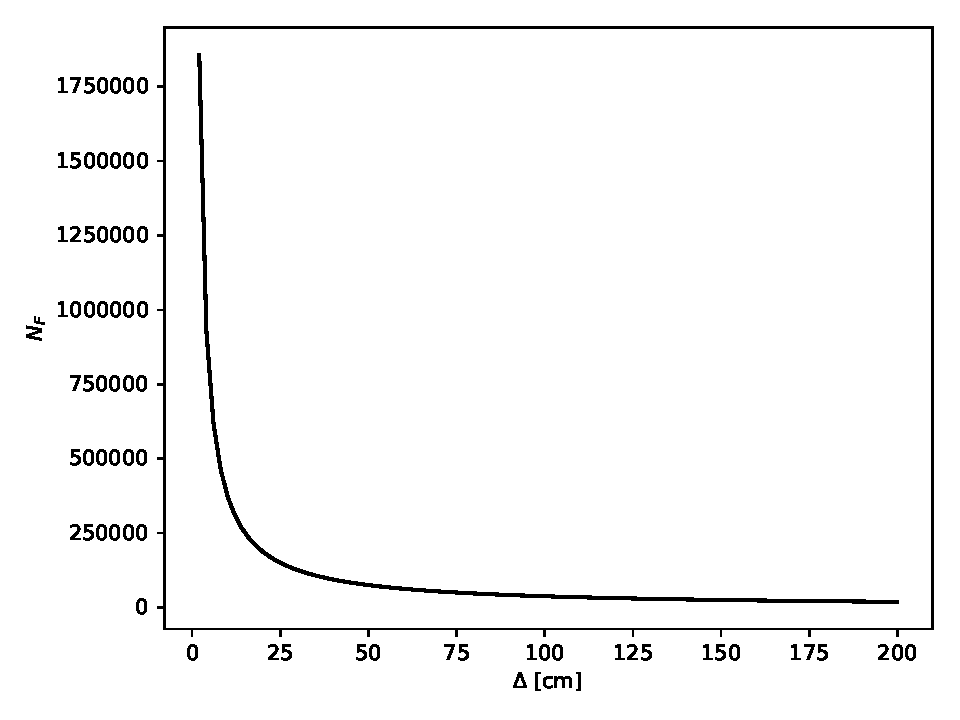
\includegraphics[width=0.6\linewidth]{figs/fresnelnum}
  \captionsetup{width=0.6\linewidth}
  \caption{Fresnel number as a function of propagation distance.}
  \label{fig:fresnelnum}
\end{figure}
We see that with these values, $N_F \gg 1$ for reasonable propagation distances,
indicating that we are safe to assume we are in the ``near'' field regime.

\section{Conclusion}

We are now ready to write down a full forward-model for our imaging system using
(admittedly loose) operator notation:
\begin{align}
  I_{\omega}(x,y,z=z_0 + \Delta) = \left|\mathcal{D}^{(\text{fs})}_{\Delta}\mathcal{D}^{(\text{sc})}_{z_0}n_{\omega}(x,y,z)\right|^2. 
\end{align}
Here, $n_{\omega}(x,y,z)$ is the 3D, complex, frequency-dependent index of
refraction of a scattering object defined between the planes $z=0$ and
$z=z_0$. $\mathcal{D}_{z_0}^{(\text{sc})}$ is a diffraction operator that
propagates an incoming monochromatic wave-field $\psiom(x,y,z=0)$ through the
scattering object to the plane $z=z_0$. This could take the form of a number of
approximations discussed in these notes: namely
equations~\ref{eq:projectionapproximation}
(projection),~\ref{eq:firstbornapproximation} (first Born),~\ref{eq:bornseries}
(Born series), or~\ref{eq:multisliceapproximation}
(multislice). $\mathcal{D}_{\Delta}^{(\text{fs})}$ is an additional diffraction
operator that propagates the scattered wave-field a distance $\Delta$ through
free space from the exit plane $z=z_0$ to the detector plane $z=z_0 + \Delta$.
This could take the form of equations~\ref{eq:freespace} (exact
solution),~\ref{eq:fresnel} (Fresnel), or~\ref{eq:fraunhofer} (Fraunhofer),
depending on various approximations discussed previously. The intensity is then
detected as the complex modulus of the wave-field at the detector plane,
integrated over the acquisition time. Note that while this analysis was
performed with respect to an incoming monochromatic wave, the results can easily
be extended to a polychromatic wave-field by modeling the frequency-dependent
detector response and integrating over all polychromatic components.

I will now begin work to set up a computational framework to generate realistic
digital phantoms and apply these various approximate propagators.  This will
allow me to explore how sensitive the different models are to the object
composition and imaging geometry. I have also begun an additional set of notes
documenting methods in the literature for linearizing these models for detected
intensity with respect to the absorption and accumulated phase imparted to the
wave-field by the object (including Paganin, chapter 4). Once I have a good
grasp of what sort of approximations are made in the literature, I will perform
additional computational studies to evaluate their suitability to our problem.

\appendix
\section{Refractive index}\label{refractindex}
We commonly express the refractive index for x-rays as
\begin{align}
  n_{\omega} = 1 - \delta_{\omega} + i\beta_{\omega},
\end{align}
where $\delta_{\omega}$ and $\beta_{\omega}$ are both $\ll 1$ in
magnitude. Evaluating $1 - n_{\omega}^2(x,y,z)$ and keeping only terms to first
order in $\delta_{\omega}$ and $\beta_{\omega}$, we have
\begin{align}
  1 - n_{\omega}^2(x,y,z) \approx 2\left[\delta_{\omega}(x,y,z) - i\beta_{\omega}(x,y,z)\right].
  \label{eq:238}
\end{align}

To evaluate this approximation, we can express the complex index of refraction
in terms of physical parameters for some material $i$:
\begin{align}
  n^{(i)}_{\omega} \approx 1 - \frac{n_a^{(i)} r_e \lambda_{\omega}^2}{2\pi}\left(f_{1,\omega}^{(i)} - if_{2,\omega}^{(i)}\right).
\end{align}
where $n_a$ is the atomic number density of the material, $r_e$ is the classical
electron radius, $\lambda$ is the x-ray wavelength, and $f_1$ and $f_2$ are the
atomic form factors tabulated by NIST.\footnote{Most derivations I have seen for
  the tabulated form factors assume a soft x-ray regime, but I believe it also
  remains valid for small-angle scattering in the hard x-ray regime (see
  \cite{Kirz1995}). We are already making the paraxial approximation, so this
  might be ok, but I want to look a bit deeper into where this expression comes
  from to be sure. NIST also has extensive documentation on the limitations and
  uncertainties in different energy regimes, which I will review.}

We thus have
\begin{align}
  \delta_{\omega}^{(i)} &= \frac{n_a^{(i)}r_e\lambda_{\omega}^2}{2\pi}f_{1,\omega}^{(i)} & \beta_{\omega}^{(i)} &= \frac{n_a^{(i)}r_e\lambda_{\omega}^2}{2\pi}f_{2,\omega}^{(i)}.
\end{align}
Note that we can calculate the atomic number density from the physical density
$\rho$ and molar mass $M_a$:
\begin{align}
  n_a^{(i)} = \frac{\rho^{(i)}N_a}{M_a^{(i)}},
\end{align}
where $N_a$ is Avogadro's number. Using nominal values for all physical
parameters, the real and complex components of the index of refraction are shown
in Figure~\ref{fig:refindex} for osmium and uranium. We see that both metals
have both components $<10^{-3}$ for relevant energy ranges, so the approximation
in equation~\ref{eq:238} is valid.

\begin{figure}[h]
  \centering
  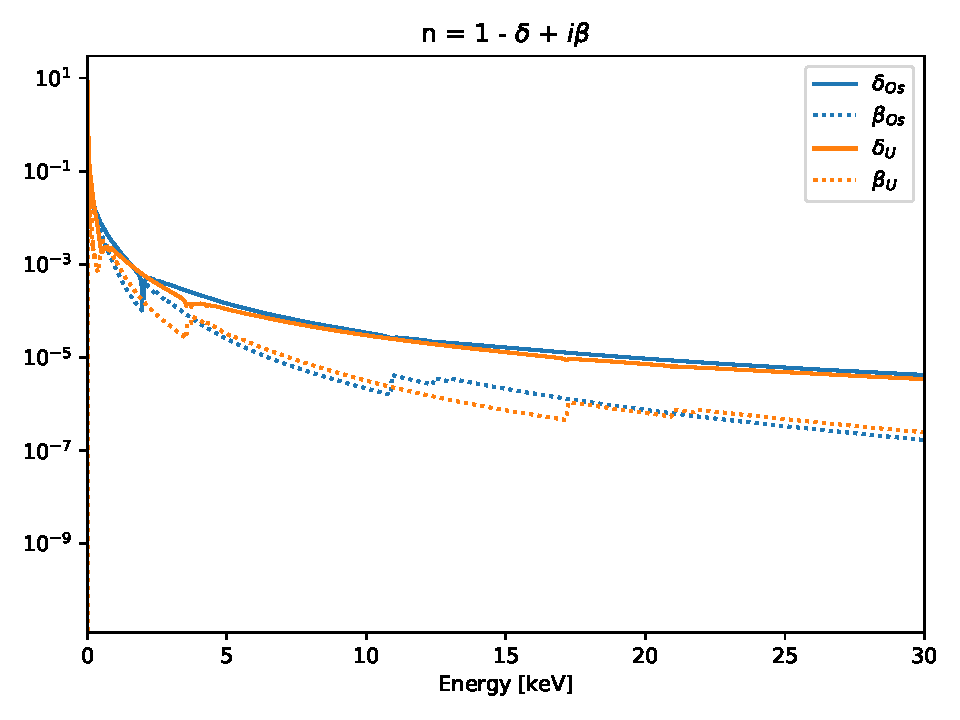
\includegraphics[width=0.6\linewidth]{figs/refindex}
  \captionsetup{width=0.6\linewidth}
  \caption{Real (solid) and imaginary (dashed) components of the complex
    index of refraction for osmium and uranium.}
  \label{fig:refindex}
\end{figure}

This formulation allows us to redefine our object as the real distribution of
physical or atomic densities, after decomposing the object into a set of known
materials (osmium and uranium, for instance).

As an example, consider the projection approximation in
equation~\ref{eq:236}. This can be written as:
\begin{align}
  \tilde{\psi}_{\omega}(x,y,z_0) &\approx \exp\left\{-ik\int_0^{z_0} \left[\delta_{\omega}(x,y,z) - i\beta_{\omega}(x,y,z)\right] \mathrm{d}z\right\}\tilde{\psi}_{\omega}(x,y,0)\nonumber\\
                                 &\approx \exp\left\{-ik\left(\frac{r_e\lambda_{\omega}^2}{2\pi}\right)\int_0^{z_0} \sum_i^N \left[\left(f_{1,\omega}^{(i)} - if_{2,\omega}^{(i)}\right)n_a^{(i)}(x,y,z)\right] \mathrm{d}z\right\}\tilde{\psi}_{\omega}(x,y,0)\nonumber\\
                                 &\approx \exp\left\{-i r_e \lambda_{\omega}\int_0^{z_0} \sum_i^N \left[\left(f_{1,\omega}^{(i)} - if_{2,\omega}^{(i)}\right)n_a^{(i)}(x,y,z)\right] \mathrm{d}z\right\}\tilde{\psi}_{\omega}(x,y,0).
\end{align}

\section{Fourier Transform}\label{Fourier}
Note that in these notes I am using the same convention as Paganin for the
2D Fourier transform:
\begin{align}
  F(k_x,k_y) = \mathcal{F}f(x,y) &= \frac{1}{2\pi}\iint_{-\infty}^{\infty} f(x, y)\exp\left[-i(k_x x + k_y y)\right] \mathrm{d}x \mathrm{d}y\\
  f(x,y) = \mathcal{F}^{-1}F(k_x, k_y) &= \frac{1}{2\pi}\iint_{-\infty}^{\infty} F(k_x, k_y)\exp\left[i(k_x x + k_y y)\right] \mathrm{d}k_x \mathrm{d}k_y
\end{align}

\bibliographystyle{ieeetr}
\bibliography{forward_model}

\end{document}